% This is LLNCS.DEM the demonstration file of
% the LaTeX macro package from Springer-Verlag
% for Lecture Notes in Computer Science,
% version 2.4 for LaTeX2e as of 16. April 2010
%
\documentclass{llncs}
%
\usepackage{makeidx}  % allows for indexgeneration
\usepackage{fancyvrb}
\usepackage{amsmath}
\usepackage{graphicx}
\usepackage{caption}
\usepackage{subcaption}
\usepackage{wrapfig}
\usepackage{nth}
\usepackage[backref,pageanchor=true,plainpages=false, pdfpagelabels, bookmarks,bookmarksnumbered]{hyperref}
\usepackage{latexsym}
\usepackage{amssymb}            % for \multimap (-o)
\usepackage{stmaryrd}           % for \binampersand (&), \bindnasrepma (\paar)

\newcommand{\m}[1]{\mathsf{#1}}
\newcommand{\f}[1]{\framebox{#1}}

\newcommand{\eph}{\mathit{eph}}
\newcommand{\pers}{\mathit{pers}}
\newcommand{\um}[1]{\underline{\m{#1}}}

\newcommand{\seq}{\vdash}
\newcommand{\semi}{\mathrel{;}}
\newcommand{\lequiv}{\mathrel{\dashv\vdash}}

% symbols of linear logic
\newcommand{\lolli}{\multimap}
\newcommand{\tensor}{\otimes}
\newcommand{\with}{\mathbin{\binampersand}}
\newcommand{\paar}{\mathbin{\bindnasrepma}}
\newcommand{\one}{\mathbf{1}}
\newcommand{\zero}{\mathbf{0}}
\newcommand{\bang}{{!}}
\newcommand{\whynot}{{?}}
\newcommand{\bilolli}{\mathrel{\raisebox{1pt}{\ensuremath{\scriptstyle\circ}}{\lolli}}}
% \oplus, \top, \bot



\begin{document}
\newcommand{\cmu}{\ensuremath{^\dag}}
\newcommand{\fcup}{\ensuremath{^\ddag}}
\pagestyle{headings}  % switches on printing of running heads
\title{A Parallel Virtual Machine for Executing Forward-Chaining Linear Logic Programs}

\titlerunning{A Parallel Virtual Machine for Executing Forward-Chaining Linear Logic Programs}


\author{Flavio Cruz\inst{1}\inst{2} \and Ricardo Rocha\inst{2}
Seth Goldstein\inst{1} \and Frank Pfenning\inst{1}}

\authorrunning{Flavio Cruz et al.} % abbreviated author list (for running head)

\institute{Carnegie Mellon University, Pittsburgh, PA 15213, USA,\\
\email{\{fmfernan, seth, fp\}@cs.cmu.edu}
\and
CRACS \& INESC TEC, Faculty of Sciences, University Of Porto\\
Rua do Campo Alegre, 1021/1055, 4169-007 Porto, Portugal\\
\email{\{flavioc, ricroc\}@dcc.fc.up.pt}}

\maketitle              % typeset the title of the contribution

\begin{abstract}
Linear Meld is a concurrent forward-chaining linear logic programming language where logical facts can be asserted and
retracted in a structured way. The database of facts is partitioned by the nodes of a graph structure and concurrency is achieved by
executing nodes simultaneously. Communication arises whenever nodes send facts to other nodes by fact derivation.
We present an overview of the virtual machine that we implemented to run Linear Meld on multicores, including
code organization, thread management, rule execution and database organization for efficient fact insertion, lookup and deletion.
Although our virtual machine is a work-in-progress, our results show that Linear Meld is not only capable of scaling graph and machine
learning programs but it also exhibits some interesting performance results when compared against other programming languages.
\keywords{linear logic programming, virtual machine, implementation}
\end{abstract}

\section{Introduction}
Logic programming is a declarative programming paradigm that has been used to advance the state of parallel programming.
Since logic programs are declarative, they are much easier to parallelize than imperative programs. First, logic programmers do not
need to use low level programming constructs such as locks or semaphores to coordinate parallel execution, because logic
systems hide such details from the programmer. Second, logic programs are easier to reason about since they are based on logical
foundations, making it easier to prove that a program is correct.

Logic based programming languages split into two main camps: forward-chaining programming languages and backwards-chaining 
programming languages. Backwards-chaining logic programs are composed of a set of rules that can be activated by inputing a query. Given a query $q(\hat{x})$, an interpreter will work backwards by matching $q(\hat{x})$ against the head of a rule. If found, the interpreter will then try to match the body of the rule, recursively, until it finds the program axioms (rules without body). If the search procedure succeeds, the interpreter finds a valid substitution for the $\hat{x}$ variables. A popular backwards-chaining programming
language is Prolog~\cite{Colmerauer:1993:BP:154766.155362}, which has been a productive research language for executing logic
programs in parallel. Researchers took advantage of Prolog's non-determinism to evaluate subgoals
in parallel with models such as \emph{or-parallelism} and \emph{and-parallelism}~\cite{Gupta:2001:PEP:504083.504085}.

In a forward-chaining logic programming language, we start with a database of facts (filled with the program's
axioms) and a set of logical rules. Then, we use the facts of the database to fire the program's rules and derive new facts that are
then added to the database. This process is repeated many times until the database reaches \emph{quiescence} and no more information can
be derived from the program.
A popular forward-chaining programming language is Datalog~\cite{Ramakrishnan93asurvey}.

In this paper, we present a new forward-chaining logic programming language called Linear Meld (LM) that is specially suited
for concurrent programming over graphs. LM differs from Datalog-like languages because it integrates both classical
logic and linear logic into the language, allowing some facts to be retracted and asserted in a logical fashion. Although most
Datalog and Prolog-like programming languages allow some kind of state manipulation~\cite{Liu98extendingdatalog}, those features
are extra-logical and do not provide a structured way to manage state like linear logic provides.

The roots of LM are the P2 system~\cite{Loo-condie-garofalakis-p2} and the original Meld~\cite{ashley-rollman-derosa-iros07wksp,ashley-rollman-iclp09}.
P2 was a Datalog-like language that mapped a computer network
to a graph, where each computer node could perform computations locally and communicate with neighbors.
Meld was itself inspired in the P2 system but adapted to the concept of massively distributed systems
made of modular robots with a dynamic topology.

LM also follows the same graph model of computation, but, instead, applies it to parallelize graph-based problems such as
graph algorithms, search algorithms and machine learning algorithms. LM programs are naturally concurrent since the graph of nodes
can be partitioned to be executed by different workers.
To realize LM, we have implemented a compiler and a virtual machine that executes LM programs on multicore machines
\footnote{Source code is available at \url{http://github.com/flavioc/meld}.}.

This paper describes the current implementation of
our virtual machine and is organized as follows: in the next section we
briefly describe LM language; in Section~\ref{virtual_machine} we present the virtual machine organization, including code organization, thread management and
execution; finally, in Section~\ref{results} we present some experimental results.

\section{The LM Language}\label{lm_language}
\newcommand{\selector}[0]{[~S~\Rightarrow~y;~BE~] \lolli HE}
\newcommand{\comprehension}[0]{\{~\widehat{x};~BE;~SH~\}}
\newcommand{\aggregate}[0]{[~A~\Rightarrow~y;~\widehat{x};~BE;~SH_1;~SH_2~]}

Linear Meld (LM) is a logic programming language that offers a declarative and structured way to manage state.
A program consists of a database and a set of derivation rules. The database consists of either persistent facts
or linear facts. Persistent facts are never deleted, while linear facts can be retracted.

The dynamic (or operational) semantics of LM are identical to Datalog.
Initially, we populate the database with the program's axioms and then determine which derivation rules can be applied by using the current database. Once a rule is applied, we derive new facts, which are then added to the database.
If a rule uses linear facts, they are deleted from the database.
The program stops when we reach \emph{quiescence}, that is, when we can no longer apply any derivation rule.

Each fact is a predicate on a tuple of \emph{values}, where the type of the predicate prescribes the types of the arguments.
LM rules are type-checked using the predicate declarations in the header of the program. LM has a simple type system that includes types such as
\emph{node}, \emph{int}, \emph{float}, \emph{string}, \emph{bool}. Recursive types such as \emph{list X} and \emph{pair X; Y} are
also allowed.

Each rule in LM has a defined priority that is inferred from its position in the source file.
Rules at the beginning of the file have higher priority. We consider all
the new facts that have been not considered yet to create a set of \emph{candidate rules}.
The set of candidate rules is then applied (by priority) and updated as new facts are derived.


{\scriptsize
\begin{figure}[h]
   \vspace{-0.5\intextsep}
\scriptsize\begin{Verbatim}[numbers=left]
type left(node, node).
type right(node, node).
type linear value(node, int, int).
type linear replace(node, int, int).

// we found our key
replace(A, K, New), value(A, K, Old)
   -o value(A, K, New).

// go left
replace(A, RKey, RValue), value(A, Key, Value), !left(A, B), RKey < Key
   -o value(A, Key, Value), replace(B, RKey, RValue).

// go right
replace(A, RKey, RValue), value(A, Key, Value), !right(A, B), RKey > Key
   -o value(A, Key, Value), replace(B, RKey, RValue).

// binary tree configuration
value(@3, 3, 3). !left(@3, @1). !right(@3, @5).
value(@1, 1, 1). !left(@1, @0). !right(@1, @2).
value(@0, 0, 0).
value(@2, 2, 2).
value(@5, 5, 5). !left(@5, @4). !right(@5, @6).
value(@4, 4, 4).
value(@6, 6, 6).

// replace value of key 6 to 7
replace(@3, 6, 7).
\end{Verbatim}
\caption{Binary tree dictionary: replacing a key's value.}
  \label{code:btree_replace}
  \vspace{-\intextsep}
\end{figure}
}

\subsection{Example}

We now present an example LM program in Fig.~\ref{code:btree_replace} that implements the key update operation for a binary tree
represented as a key/value dictionary.
We first declare all the predicates (lines 1-4), which represent the kinds of facts we are going to use.
Predicate \texttt{left/2} and \texttt{right/2} are persistent while \texttt{value/3} and \texttt{replace/3} are linear.
\texttt{value/3} assigns a key/value pair to a binary tree node and can
be updated since it is linear. The \texttt{replace/3} linear predicate represents an update operation where the key in
the second argument will be updated to the value in the third argument.

The algorithm uses three rules for the three cases of updating a key's value: the first rule (lines 6-8) performs the update;
the second rule (lines 10-12) recursively picks the left branch for the update operation; and the third rule (lines 14-16) picks the right branch.
The axioms of this program are presented in lines 18-28 and they describe the initial binary tree configuration, including keys and values.
By having the \texttt{update(@3, 6, 7)} axiom instantiated at the root node we intend to change the the value of key 6 to 7.
Note that when writing rules or axioms we precede persistent facts with a \texttt{!}.

Fig.~\ref{fig:btree_trace} represents the trace of the algorithm. Note that the program database has been partitioned
by the tree nodes using the first argument of each fact. In Fig.~\ref{fig:btree_trace}~(a) we present the database
filled with the program's axioms. Next, we follow the right branch using rule 3 since $6 > 3$ (Fig.~\ref{fig:btree_trace}~(b)).
We use the same rule again in Fig.~\ref{fig:btree_trace}~(c) where we finally reach the key 6. Here, we apply rule 1 and
\texttt{value(@6, 6, 6)} is updated to \texttt{value(@6, 6, 7)}.

\begin{figure}[h]
   \vspace{-0.75\intextsep}
        \centering
        \begin{subfigure}[b]{0.5\textwidth}
                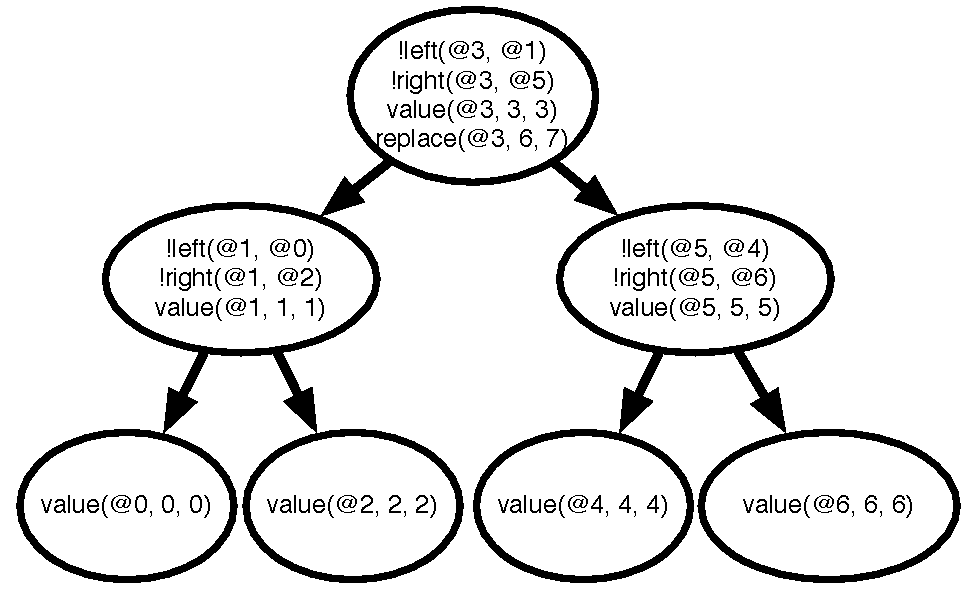
\includegraphics[width=\textwidth]{btree_trace1}
                \caption{Initial database. Replace axiom instantiated at the $@3$ root node.}
                \label{fig:btree_trace1}
        \end{subfigure}%
        ~
        \begin{subfigure}[b]{0.5\textwidth}
                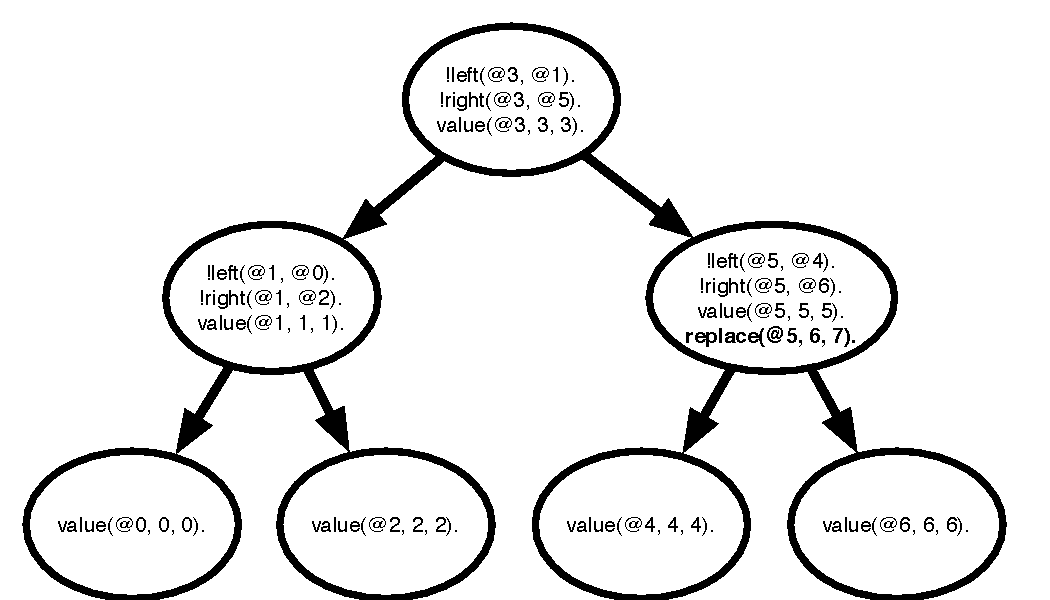
\includegraphics[width=\textwidth]{btree_trace2}
                \caption{After applying rule 3 at node $@3$. Replace fact sent to node $@5$.}
                \label{fig:btree_trace2}
        \end{subfigure}\\
        \begin{subfigure}[b]{0.5\textwidth}
                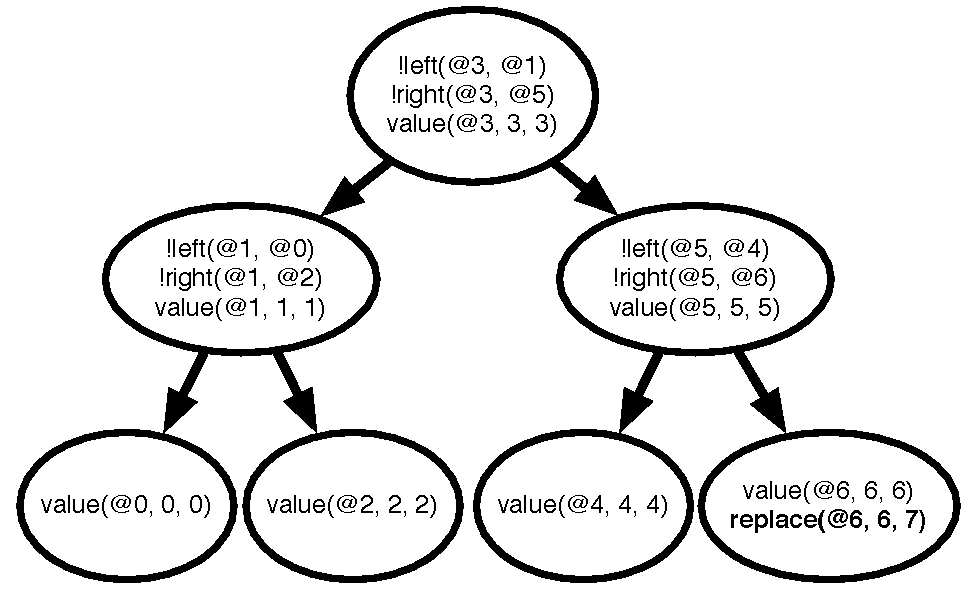
\includegraphics[width=\textwidth]{btree_trace3}
                \caption{After applying rule 3 at node $@5$. Replace fact reaches node $@6$.}
                \label{fig:btree_trace3}
        \end{subfigure}%
        ~
        \begin{subfigure}[b]{0.5\textwidth}
                  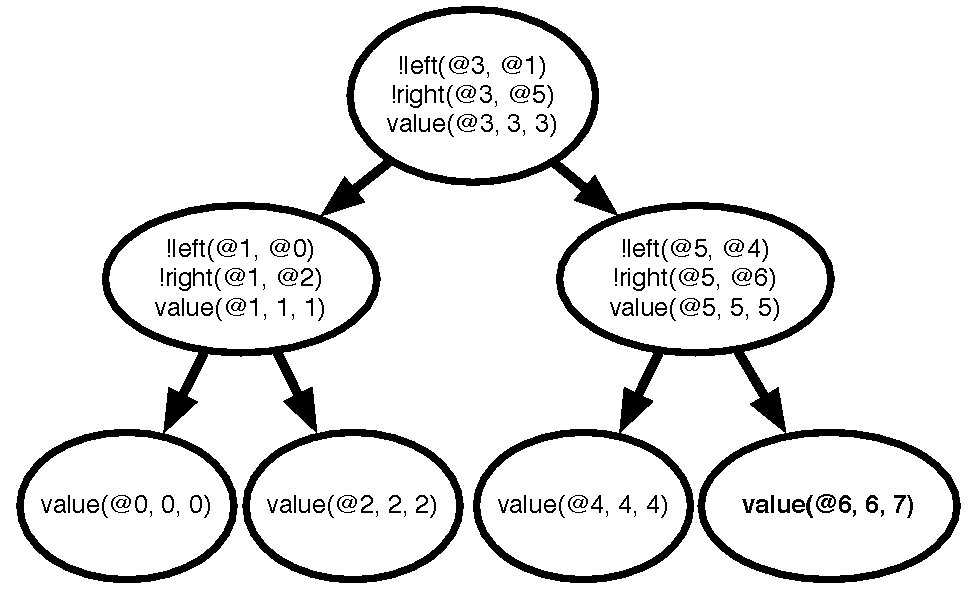
\includegraphics[width=\textwidth]{btree_trace4}
                  \caption{After applying rule 1 (nodes $@5$). Value of key 6 has changed to 7.}
                  \label{fig:btree_trace4}
          \end{subfigure}
        \caption{An execution trace for the binary tree dictionary algorithm.}\label{fig:btree_trace}
        \vspace{-\intextsep}
\end{figure}

\subsection{Syntax}

\renewcommand{\arraystretch}{1.2}
\begin{table}[h]
\centering
\begin{tabular}{ l l c l }
  Program & $Prog$ & $::=$ & $\Sigma, D$ \\
  Set Of Rules & $\Sigma$ & $::=$ & $\cdot \; | \; \Sigma, R$\\
  Database & $D$ & $::=$ & $\Gamma; \Delta$ \\
  Rule & $R$ & $::=$ & $BE \lolli HE \; | \; \forall_{x}. R$ \\
  Body Expression & $BE$ & $::=$ & $L \; | \; P \; | \; C \; | \; BE, BE \; | \; \exists_{x}. BE \; | \; 1$\\
  Head Expression & $HE$ & $::=$ & $L \; | \; P \; | \; HE, HE \; | \; CE \; | \; AE \; | \; 1$\\
  
  Linear Fact & $L$ & $::=$ & $l(\hat{x})$\\
  Persistent Fact & $P$ & $::=$ & $\bang p(\hat{x})$\\
  Constraint & $C$ & $::=$ & $c(\hat{x})$ \\
  
  Comprehension & $CE$ & $::=$ & $\comprehension$ \\
  Aggregate & $AE$ & $::=$ & $\aggregate$ \\
  Aggregate Operation & $A$ & $::=$ & $\mathtt{min} \; | \; \mathtt{max} \; | \; \mathtt{sum} \; | \; \mathtt{count}$ \\
  
  Sub-Head & $SH$ & $::=$ & $L \; | \; P \; | \; SH, SH \; | \; 1$\\
  
  Known Linear Facts & $\Delta$ & $::=$ & $\cdot \; | \; \Delta, l(\hat{t})$ \\
  Known Persistent Facts & $\Gamma$ & $::=$ & $\cdot \; | \; \Gamma, \bang p(\hat{t})$ \\
\end{tabular}
\vspace{0.5\intextsep}
\caption{Abstract syntax of LM.}
\label{tbl:ast}
\vspace{-1\intextsep}
\end{table}
\renewcommand{\arraystretch}{1.0}

Table~\ref{tbl:ast} shows the abstract syntax for rules in LM.
A LM program $Prog$ consists of a set of derivation rules $\Sigma$ and a database $D$.
Each derivation rule $R$ can be written as $BE \lolli HE$ where $BE$ is the body of a rule and
$HE$ is the head. Rules without bodies are allowed in LM and they are called \textit{axioms}. Rules without heads are also allowed.

The body of a rule, $BE$, may contain linear ($L$) and persistent ($P$) \emph{fact expressions}
and constraints ($C$). Fact expressions are template facts that instantiate variables
(from facts in the database). Variables can be used again in the body for matching and
also in the head when instantiating facts. Constraints are boolean expressions that must
be true in order for the rule to be fired. Constraints use variables from fact expressions and are built using a small functional language that includes mathematical operations, boolean operations, external functions and literal values.

The head of a rule, $HE$, contains linear ($L$) and persistent ($P$) \emph{fact templates} which are uninstantiated facts and will derive new facts. The head can also have \emph{comprehensions} ($CE$) and \emph{aggregates} ($AE$). All those expressions
may use all the variables instantiated in the body.

\subsubsection{Comprehensions}

Sometimes we need to consume a linear fact and then immediately generate several facts depending on
the contents of the database. To solve this particular need, we created the concept of comprehensions, which are
sub-rules that are applied with all possible combinations of facts from the database. In a comprehension $\comprehension$,
$\widehat{x}$ is a list of variables, $BE$ is the body of the comprehension and $SH$ is the head.
The body $BE$ is used to generate all possible combinations for the head $SH$, according to the facts
in the database.

The following example illustrates a simple program that uses comprehensions:

{\footnotesize
\begin{Verbatim}
!edge(@1, @2).
!edge(@1, @3).
iterate(@1).
iterate(A) -o {B | !edge(A, B) | perform(B)}.
\end{Verbatim}
}

When the rule is fired, we consume \texttt{iterate(@1)} and then generate the comprehension. Here, we iterate through
all the \texttt{edge/2} facts that match \texttt{!edge(@1, B)}, which are: \texttt{!edge(@1, @2)} and \texttt{!edge(@1, @3)}.
For each fact, we derive \texttt{perform(B)}, namely: \texttt{perform(@2)} and \texttt{perform(@3)}.

\subsubsection{Aggregates}

Another useful feature in logic programs is the ability to reduce several facts into a single fact.
In LM we have aggregates ($AE$), a special kind of sub-rule that works very similarly to comprehensions.
In the abstract syntax $\aggregate$, $A$ is the aggregate operation, $\widehat{x}$ is the list of variables
introduced in $BE$, $SH_1$ and $SH_2$ and $y$ is the variable in the body
$BE$ that represents the values to be aggregated using $A$. Like comprehensions,
we use $\widehat{x}$ to try all the combinations of $BE$, but, in addition to deriving $SH_1$ for each combination,
we aggregate the values represented by $y$ and derive $SH_2$ only once using $y$.

To better understand aggregates, let's consider a database with the following facts and a rule:

{\footnotesize
\begin{Verbatim}
price(@1, 3).
price(@1, 4).
price(@1, 5).
count-prices(@1).
count-prices(A) -o [sum => P | . | price(A, P) | 1 | total(A, P)].
\end{Verbatim}
}

By applying the rule, we consume \texttt{count-prices(@1)} and
derive the aggregate which consumes all the \texttt{price(@1, P)} facts.
These are summed and \texttt{total(@1,~12)} is derived.  
LM provides several aggregate operations, including the minimum, maximum, sum, and count.

\subsection{Concurrency}

LM is at its core a concurrent programming language.
The database of facts can be seen as a graph data structure where each node contains a fraction of the database.
To accomplish this, we force the first argument of each predicate to be typed as a \emph{node}. We then
restrict the derivation rules to only manipulate facts belonging to a single node.
However, the expressions in the head may refer to other nodes, as long as those nodes are instantiated in the body of the rule.

Due to the restrictions on LM rules, nodes are able to
run rules independently without using other node's facts. Node computation follows a
\emph{don't care} or \emph{committed choice} non-determinism
since any node can be picked to run as long as it contains enough facts to fire a derivation rule.
Facts coming from other nodes will arrive in order of derivation but may be considered
partially and there is no particular order among the neighborhood. To improve concurrency,
the programmer is encouraged to write rules that take advantage of the non-deterministic nature of execution.

LM has been used to implement several parallel algorithms, including: belief propagation~\cite{Gonzalez+al:aistats09paraml},
belief propagation with residual splash~\cite{Gonzalez+al:aistats09paraml}, PageRank, graph coloring,
N queens, shortest path, diameter estimation, map reduce, game of life, quick-sort, neural network training, among others.

\section{The Virtual Machine}\label{virtual_machine}

We developed a compiler that compiles programs to byte-code and a multi-threaded
virtual machine (VM) using the Pthreads library that runs the byte-code.
If we execute programs with $P$ threads, our implementation will partitions the application
graph of $N$ nodes into $P$ subgraphs and then each thread will work on their own subgraph.

The goal of our system is to keep the threads as busy as possible and to reduce inter-thread communication.
The load balancing aspect of the system is performed by our work scheduler that is based on a work
stealing algorithm. More specifically, threads can steal nodes of other threads to keep themselves busy.
Reduction of inter-thread communication is achieved by first ordering the node addresses present
in the code in such a way that closer nodes are clustered together and then partitioning them
to threads.

During compilation, we take note of predicates that are used in rules for
communication rules (arguments with type \emph{node}) and then build a graph of nodes from
the program's axioms. The nodes of the graph are then ordered by using a breadth-first search
algorithm that changes the nodes of addresses to the domain $[0, n[$, where $n$ is the number of
nodes. Once the VM starts, we simply partition the range
$[0, n[$ in order to partition the graph.

\subsection{Multicore}

When the VM starts, it reads the byte-code file and starts all threads.
As a first step, all threads will grab their nodes and assign the \texttt{owner} property of each node.
Because only one thread is allowed to do computation on a node at any giving time, the owner property
defines the thread with such permission.
Next, each thread fills up its \emph{work queue} with the initial nodes. This queue
maintains the nodes that have new facts to be processed.

The main thread loop is shown in Fig.~\ref{code:work_loop}. For every iteration of the loop, the thread inspects the work queue
for nodes to process. Procedure \texttt{process\_node} takes a node with new candidate rules and executes the rules until no more
rules are applicable. If the work queue is empty, then the thread attempts to steal of node from another thread before
becoming idle. The thread will try to find another
thread with at least one extra active node. Starting from a random thread, it cycles through all the threads
and steals from the first thread with nodes. Currently, each thread only takes one node per steal.

\begin{figure}[h!]
   \vspace{-0.2\intextsep}
\scriptsize\begin{Verbatim}
void work_loop(thread_id tid):
   while (true):
      if(has_work(tid)):
         current_node = pop_work(tid); // take node from the queue
      else:
         for (i = 0; i < NUM_THREADS; ++i): // need to steal a node
            if (current_node = steal_node_from_thread(target_thread):
               break;
            target_thread = (target_thread + 1) % NUM_THREADS;
      if(current_node == NULL):
         become_idle(tid);
         if(!synchronize_termination(tid)):
            return;
         become_active(tid);
      else:
         process_node(current_node, tid);
\end{Verbatim}
\vspace{-0.5\intextsep}
  \caption{Thread work loop.}
  \label{code:work_loop}
  \vspace{-0.5\intextsep}
\end{figure}

When a node sends a fact to another node, we need to check if the target node is in the same work queue of the owner thread.
When the two nodes are in different threads, then we have a point of synchronization. Eventually,
there will be no more work to do and the threads will go idle. There is a global atomic counter, a global
boolean flag and one boolean flag (active/idle) for each thread that are used to detect termination.
Once a thread goes idle, it decrements the global counter and changes its flag to idle. If the counter
reaches zero, the global flag is set to idle. Since every thread will be busy-waiting and checking
the global flag, they will detect the change and exit the program.

\subsection{Byte-Code}

A byte-code file contains meta-data about the program's predicates, initial nodes, partitioning
information, and code for each rule. Rule code uses a custom-made set of instructions that
use the database to match the body of the rule and then derive the head. Note that a rule
is only executed if there is a good change that it will successfully match (more details
in Section~\ref{rule_engine}).

Each VM thread has 32 registers that are used during rule execution.
Registers can store facts, integers, floats, node addresses and pointers to runtime 
data structures (lists and structures). When registers store facts, we can reference
fields in the fact through the register.

\begin{wrapfigure}{l}{0.5\textwidth}
   \vspace{-1\intextsep}
\scriptsize\begin{Verbatim}
PERSISTENT ITERATE OVER a MATCHING TO reg 0
  LINEAR ITERATE OVER b MATCHING TO reg 1
      (match).0=0.0
    LINEAR ITERATE OVER c MATCHING TO reg 2
        (match).0=0.0
        (match).1=0.1
      ALLOC d TO reg 3
      MVFIELDFIELD 0.1 TO 3.0
      ADDLINEAR reg 3
      REMOVE reg 2
      REMOVE reg 1
      RETURN DERIVED
    NEXT
  NEXT
RETURN
\end{Verbatim}
\caption{Byte-code for rule \texttt{!a(X,Y), b(X,Z), c(X,Y) -o d(Y).}}
\label{fig:byte_code}
\vspace{-1\intextsep}
\end{wrapfigure}

Given a rule \texttt{!a(X,Y), b(X,Z), c(X,Y) -o d(Y)} and a database with facts
\texttt{!a(1,2), !a(2,3), b(1,3), b(5,3), c(1,2), c(1,3), c(5,3)} rule execution proceeds
in a series of recursive loops: the first loop retrieves an iterator for the persistent facts
of the predicate \texttt{!a/2} and moves the first valid fact, \texttt{!a(1,2)},
to register 0; the inner loop retrieves linear facts that match \texttt{b(1,Z)} (from the
\emph{join constraint}) and moves \texttt{b(1,3)} to register 1; finally, in the final inner
loop we move \texttt{c(1,2)} to register 2 and the body of the rule is successfully matched. Next, we
derive \texttt{d(2)}, where \texttt{2} comes from register 0.
In Fig.~\ref{fig:byte_code} we show the concrete byte-code for the example rule.

In case of failure to find a valid fact at any given loop, we jump
to the outer loop in order to try the next candidate.
If a rule match succeeds and the head is derived, we progressively backtrack to the outer most valid loop:
if any inner loop uses linear facts we remove the fact from the database, but we will
continue backtracking until we reach the first loop that uses linear facts,
because all the others are now invalid (invalid candidates). In our example, we would jump to the
loop of \texttt{b(X,Z)} and not \texttt{c(X,Y)}, since \texttt{b(1,3)} was already consumed.

The compiler re-orders the fact expressions used in the body in order to make execution more
efficient. For example, it forces the join constraints in rules to appear at the beginning so
that matching will fail sooner rather than later. It also does the same for constraints.
Note that for every loop, the compiler adds a \emph{match object}, which contains information
about which arguments need to match, so that runtime matching is efficient.

\subsection{Database Data Structures}\label{sec:database}

We said before that LM rules are constrained by the first argument. Because nodes can execute
independently, our database is indexed by the node address and each sub-database does not
need to deal with synchronization issues since at any given point, only one thread will be using
the database. Note that the first argument of each fact is not stored.

Each (sub-)database is implemented using three data structures: trie data structures, list data structures and hash table data structures.
The database must be implemented efficiently because during matching of rules we need
to restrict the facts using a given match object, which fixes arguments of the target predicate to instantiated values. The data structures used are as follows:

\begin{itemize}
   \item \emph{Trie Data Structures} are used exclusively to store persistent facts.
   Tries are trees where facts are indexed by the common arguments. When a trie level has too many nodes, we
   transform the linked list into a hash table in order to improve lookup.
      
   \item \emph{Doubly Linked List Data Structures} are used to store linear facts.
   Each fact contains the standard \texttt{prev} and \texttt{next} pointers
   and the fact arguments. We use a double linked list because it is very efficient to add and remove facts.
   
   \item \emph{Hash Table Data Structures} are used when linked lists are too long and we need to search filter by a fixed argument. The virtual machine decides which arguments are best to be indexed
   (see Section~\ref{indexing}) and then
   uses an hash table indexed by the appropriate argument. If we need to go through all the facts, we just iterate through all the facts in the table. For collisions, we use the above doubly linked list data structure.
\end{itemize}

\begin{wrapfigure}{r}{0.5\textwidth}
   \vspace{-1\intextsep}
   \centering
   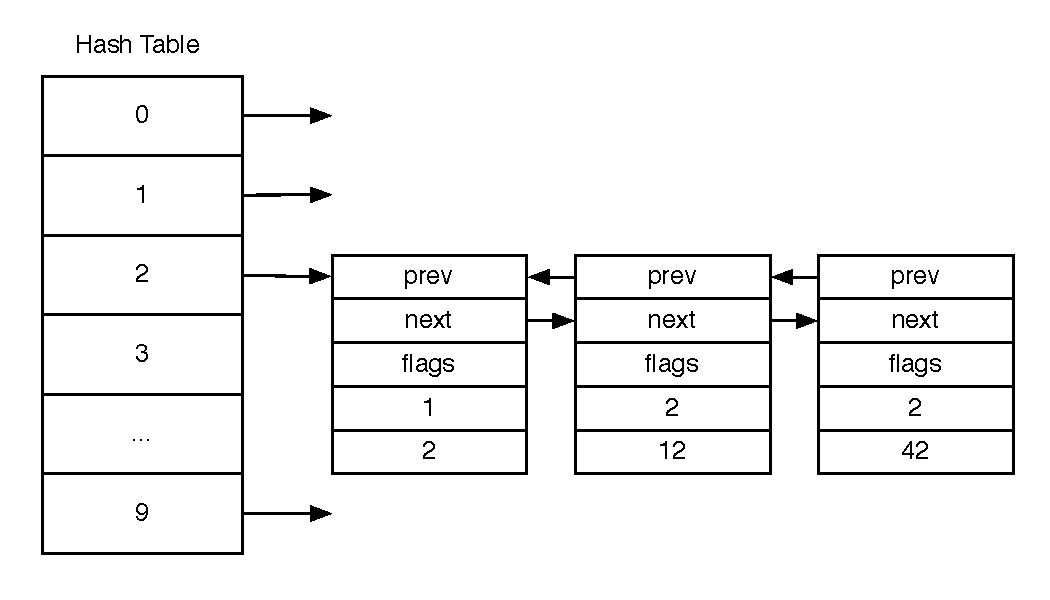
\includegraphics[width=0.48\textwidth]{hash_table.pdf}
   \caption{Example hash table data structure for storing predicate \texttt{a(int,int)}.}
   \label{fig:hash_table}
   \vspace{-1.5\intextsep}
\end{wrapfigure}

In Fig.~\ref{fig:hash_table} we show an example hash table data structure storing predicate \texttt{a(int,int)}. The table
has 10 buckets and indexes facts by the second argument. We show the doubly linked list for bucket \texttt{2}. Each linear fact
contains the regular list pointers, the fact arguments and a \texttt{flags} field. Those are all stored continuously to improve data
locality. One use of the \texttt{flags} field is to mark that a fact is already being used. For example,
consider the rule body \texttt{a(A,B), a(C,D) -o ...}. We first pick a fact for \texttt{a(A, B)} from the hash table, then we mark it as
being used and when we retrieve facts for \texttt{a(C, D)}, we know that one of them cannot be used because it would
violate linearity.

\subsection{Rule Engine}\label{rule_engine}

The rule engine decides which rules may need to be executed while taking into account rule priorities.
In Fig.~\ref{fig:rule_engine} we present the 5 main data structures for scheduling rule execution.
\texttt{Rule Queue} is the bitmap representing the rules that will be run, \texttt{Active Bitmap} contains the rules that have enough
facts to be fired, \texttt{Inactive Bitmap} contains the rules that must be dropped from \texttt{Rule Queue}, \texttt{Predicates Bitmap}
marks the newly derived facts and \texttt{Predicates Count} counts the number of facts per predicate.
To understand how our engine works, consider
the program in Fig.~\ref{code:5rules}.

\begin{wrapfigure}{l}{0.3\textwidth}
\vspace{-1\intextsep}
\footnotesize\begin{Verbatim}
a, e(1) -o b.
a -o c.
b -o d.
e(0) -o f.
c -o e(1).
\end{Verbatim}
\caption{\small{Example program with 5 rules.}}
\label{code:5rules}
\vspace{-0.5\intextsep}
\end{wrapfigure}

To apply the rules, we take the least significant rule from the bitmap, which is the candidate rule with the higher priority, and then run it. In our example, we need to execute the second rule \texttt{a -o c}, since we have facts \texttt{a} and \texttt{e(0)}.
Because the derivation is successful, we derive \texttt{c} and consume \texttt{a}. In Fig.~\ref{fig:rule_engine}~(b) we
activate the \texttt{c} predicate in the \texttt{Predicates Bitmap} since it was derived and then activate the first and second rules
in \texttt{Dropped Bitmap} since such rules are no longer applicable (\texttt{a} is gone). To update the \texttt{Rule Queue},
we remove the bits marked in \texttt{Dropped Bitmap} and add the active rules marked in \texttt{Active Bitmap} that are affected
by predicates in \texttt{Predicates Map}. The engine has now scheduled the fourth and fifth rules to be run.

Note that every node in the program has the same set of data structures present in Fig.~\ref{fig:rule_engine}.
We use 32 bits integers to implement bitmaps and an array of 16 bits integers to count facts, resulting in
$32 + 2P$ bytes per predicate.

\begin{figure*}[h]
   \vspace{-\intextsep}
   \centering
   \begin{subfigure}[b]{0.45\textwidth}
      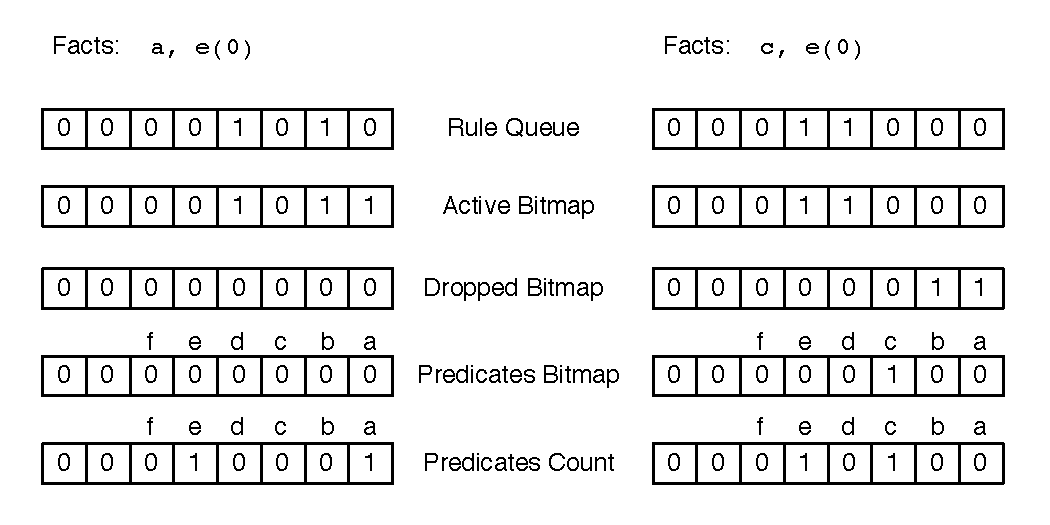
\includegraphics[width=\textwidth]{rule_queue1.pdf}
      \caption{Before applying the second rule.}
   \end{subfigure}
   \begin{subfigure}[b]{0.45\textwidth}
      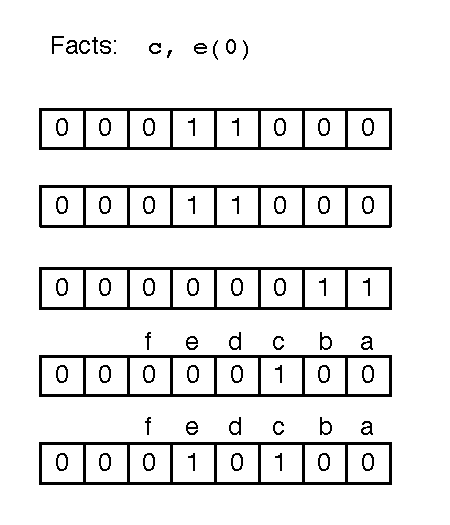
\includegraphics[width=\textwidth]{rule_queue2.pdf}
      \caption{After applying the second rule.}
   \end{subfigure}
   \caption{Rule engine main data structures.}
   \label{fig:rule_engine}
   \vspace{-0.5\intextsep}
\end{figure*}

We do a small optimization to reduce the number of derivations of persistent facts. We
divide the program rules into two sets: \emph{persistent rules} and \emph{non persistent rules}.
Persistent rules are rules where only persistent facts are involved. We compile such rules
incrementally, that is, we attempt to fire all rules where a persistent fact is used. This is called
the \emph{pipelined semi-naive} evaluation and it originated in the P2 system~\cite{Loo-condie-garofalakis-p2}.
This evaluation method avoids excessing re-derivations of the same fact. The order of derivation does not matter for those rules, since
only persistent facts are used.

\subsubsection{Thread Interaction}

Whenever a node derives a new fact through rule derivation, we need to update the data structures of the rule engine.
This is trivial if done by the thread that owns the node, however, if a thread $T1$ executes a node and a fact is derived
at a node owned by another thread $T2$, then we may have problems because $T2$ may be also updating the data structures.
We added a lock and a boolean flag to each node to protect the access to the data structures. When a node starts to execute,
we activate the flag and lock the node. When another thread tries to use the data structures, if first checks the flag and if
not activated, it locks the node and performs the required updates. If the flag is activated, it stores the newly created fact
on a list of facts that is processed before the node is executed.

\subsection{Indexing}\label{indexing}

In Section~\ref{rule_engine} we explained that we use hash tables to dynamically index facts.
The VM employs a fully dynamic mechanism to decide which argument may be optimal to improve fact lookup.
The algorithm is performed in the initial part of the program execution and empirically tries to assess the argument
of each predicate that more equally spreads the database across the values of the argument. Note that only one thread
performs the algorithm.

The indexing algorithm is performed in three main steps. First, it gathers statistics of lookup data by keeping a counter
of each predicate's argument.
Every time a fact search is performed where arguments are fixed to a value, the counter of such arguments is incremented. This phase is performed during rule execution of $1/25n$ nodes, where $n$ is the number of nodes in the program.

The second step of the algorithm initially decides the candidate arguments of each predicate.
If a predicate did not fix any arguments, then it will be not indexed.
If only one argument was fixed, then such such argument is set as the indexing argument. Otherwise, the top 2 arguments
are selected for the third phase, where \emph{entropy statistics} are collected dynamically.

During the third phase, each candidate argument has an entropy score.
Before a node is executed, the facts of the target predicate
are used in the following formula applied for the two arguments:

\vspace{-0.5\intextsep}

\[
Entropy(A, F) = - \sum_{v \in values(F, A)} \frac{count(F, A = v)}{total(F)} 	\log_2 \frac{count(F, A = v)}{total(F)}
\]
\vspace{-0.5\intextsep}

Where $A$ is the target argument, $F$ is the multi-set of linear facts for the target predicate, $values(F, A)$ is set of values of the argument $A$, $count(F, A = v)$ counts the number
of linear facts where argument $A$ is equal to $v$ and $total(F)$ counts the number of linear facts in $F$.
The entropy value is a good metric because it tells us how much information is needed to describe an argument.
If more information is needed, then that must be the best argument to index.

For one of the arguments to score, $Entropy(A, F)$ multiplied by the number of times it has been used for lookup must be larger than the other argument. This is performed for $1/25n$ node executions.

In the final and third phase, the best argument with the best score is selected and then
a global variable called \texttt{indexing\_epoch} is updated.
In order to convert the node's linked lists into hash tables, each node has local variable also called \texttt{indexing\_epoch}
that is compared to the global variable in order to rebuild the node database according to the new indexing
information.

Our VM also dynamically resizes the hash table to accommodate every increasing or decreasing hash tables. When the hash table becomes
too dense, the hash table becomes twice as big. When it becomes too sparse, the table is reduce in half
or simply transformed back into a doubly linked list. This is done once in a while, before a node executes.

In our experience, we have seen very good results with this scheme, with programs such as the all-pairs shortest paths with a 2 to 5-fold
improvement in speed. The overhead of dynamic indexing is also negligible since programs run almost as fast
as if the indices have been added from the start.

\begin{wrapfigure}{r}{0.5\textwidth}
\vspace{-1.5\intextsep}
\scriptsize\begin{Verbatim}
LINEAR ITERATE OVER a MATCHING TO reg 0
  MVFIELDREG 0.0 TO reg 1
  MVINTREG INT 1 TO reg 2
  reg 1 INT PLUS reg 2 TO reg 3
  MVREGFIELD reg 3 TO 0.0
  UPDATE reg 0
  RETURN DERIVED
RETURN
\end{Verbatim}
\caption{\small{Byte-code for rule \texttt{a(N) -o a(N+1)}.}}
\label{code:update}
\vspace{-1.5\intextsep}
\end{wrapfigure}

\subsection{Update Optimization}

Our compiler also detects cases where we re-derive a linear fact with new arguments.
For example, as shown in Fig.~\ref{code:update}, the rule \texttt{a(N) -o a(N+1)}
will compile to code that reuses the old \texttt{a(N)} fact.
We use the \texttt{flags} field presented in Section~\ref{sec:database} to mark updated nodes.

\iffalse

\subsection{Runtime Data Structures}

LM supports recursive types such as lists and pairs. These complex data structures are stored in
the heap of the VM and are managed through reference counting. For instance, each list
is a \emph{cons cell} with 3 fields: \texttt{tail}, the pointer to the next element of the list;
\texttt{head}, the element stored by this element of the list; and \texttt{refs} that counts the
number of pointers to this list element in the VM. The list is deleted from the heap whenever
\texttt{refs} is decremented to 0.

\fi

\section{Preliminary Results}\label{results}
This section presents preliminary results for our VM.
First, we present scalability results in order to show that LM programs can take advantage of multicore architectures.
Next, we present a comparison with similar programs written in other programming languages
in order to show evidence that our VM is viable.

For our experimental setup, we used a machine 
with two 16 (32) Core AMD Opteron
(tm) Processor 6274 $@$ 2.2 GHz with 32 GBytes of RAM memory and running the Linux
kernel 3.8.3-1.fc17.x86\_64.
     We compiled our VM using GCC 4.7.2 (g++) with the flags \texttt{-O3 -std=c+0x -march=x86-64}.
     We run all experiments 3 times and then averaged the execution time.
     
\subsubsection{Scalability Results}

For this section, we run each program using 1, 2, 4, 6, 8, 10, 12, 14 and 16 threads and compared the runtime against the execution of the sequential version of the VM. We used the following programs:

\newcommand{\figsize}[0]{6.5cm}
\captionsetup[sub]{              % The subcaption settings
       font=scriptsize}

\begin{itemize}
   \item Greedy Graph Coloring (GGC) colors nodes in a graph so that no two adjacent nodes have the same color. We start with a small number of colors and then we expand the number of colors when we cannot color the graph.
   \item PageRank implements a PageRank algorithm without synchronization between iterations. Every time a node sends a new rank to its neighbors and the change was significant, the neighbors are scheduled to recompute their ranks.
   \item N-Queens, the classic puzzle for a 13x13 board.
   \item Belief Propagation, a machine learning algorithm to denoise images.
\end{itemize}

Figure~\ref{exp:graph_coloring} presents the speedup results for the GGC program using 2 different datasets. In Fig.~\ref{exp:graph_coloring}a we show the speedup for a search engine graph of 12,000 webpages\footnote{Available from \url{http://www.cs.toronto.edu/~tsap/experiments/download/download.html}}. Since this dataset follows the power law, that is, there is a small number of pages with a lots of links (1\% of the nodes have 75\% of the edges), the speedup is slightly worse than the benchmark shown in Fig.~\ref{exp:graph_coloring}b, where we use a random dataset of 2,000 nodes with an uniform distribution of edges.

\newcommand{\plotsize}{0.38\textwidth}

\begin{figure*}[h]
   \vspace{-0.7\intextsep}
   \centering
   \begin{subfigure}[b]{\plotsize}
      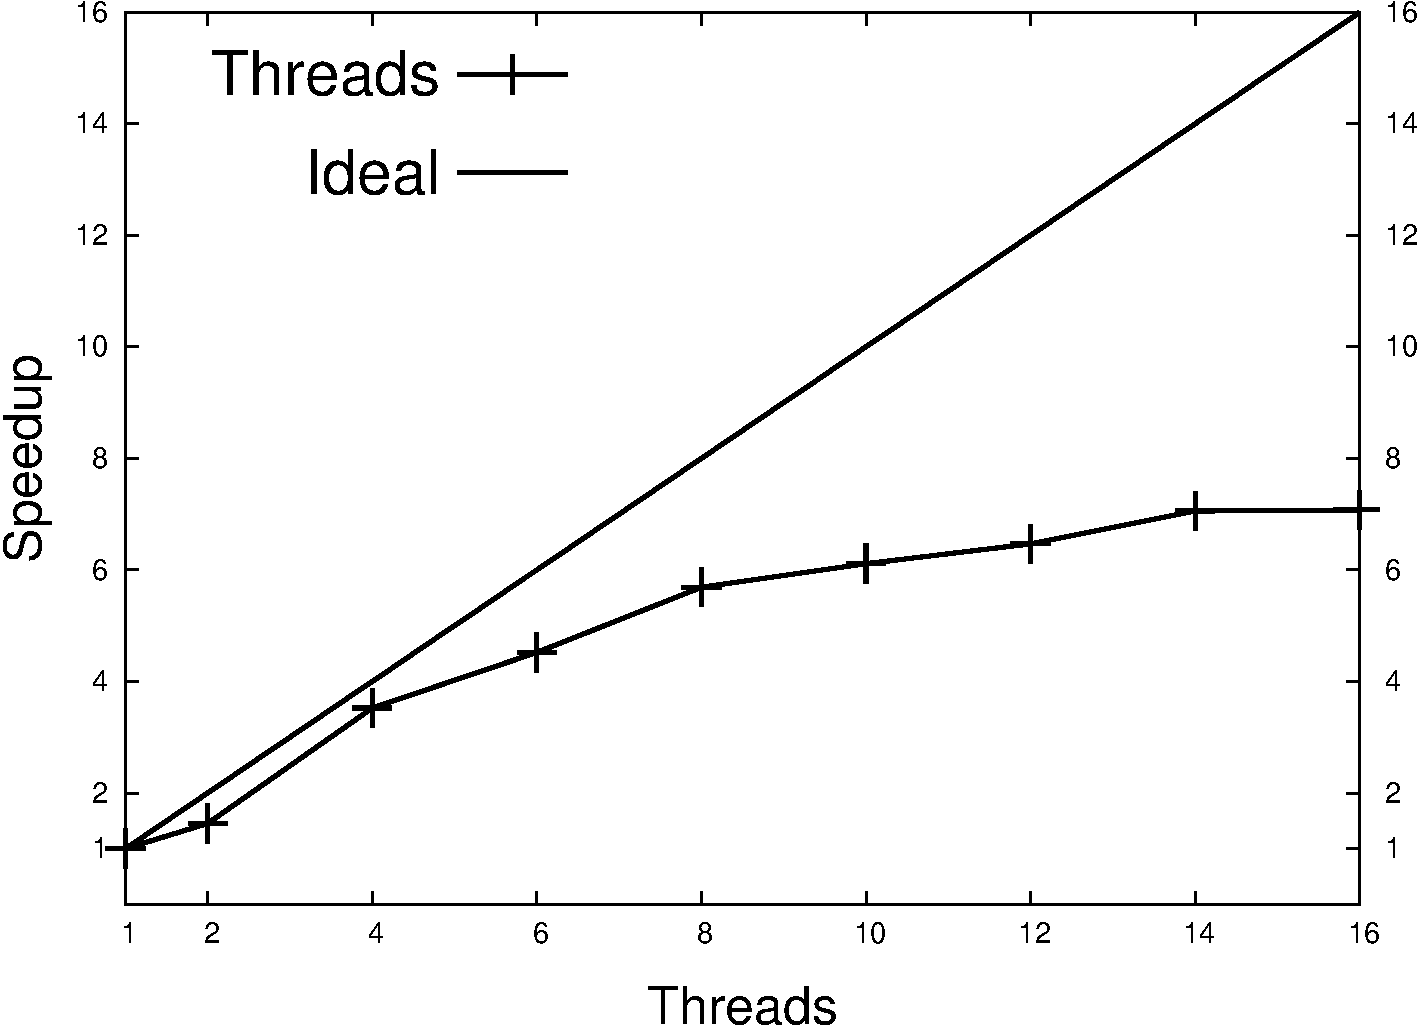
\includegraphics[width=\textwidth]{speedup_greedy-graph-coloring-search_engines.pdf}
      \caption{Using a graph of web pages with around 12,000 nodes and 292,000 edges.}
   \end{subfigure}
   ~~~~
   \begin{subfigure}[b]{\plotsize}
      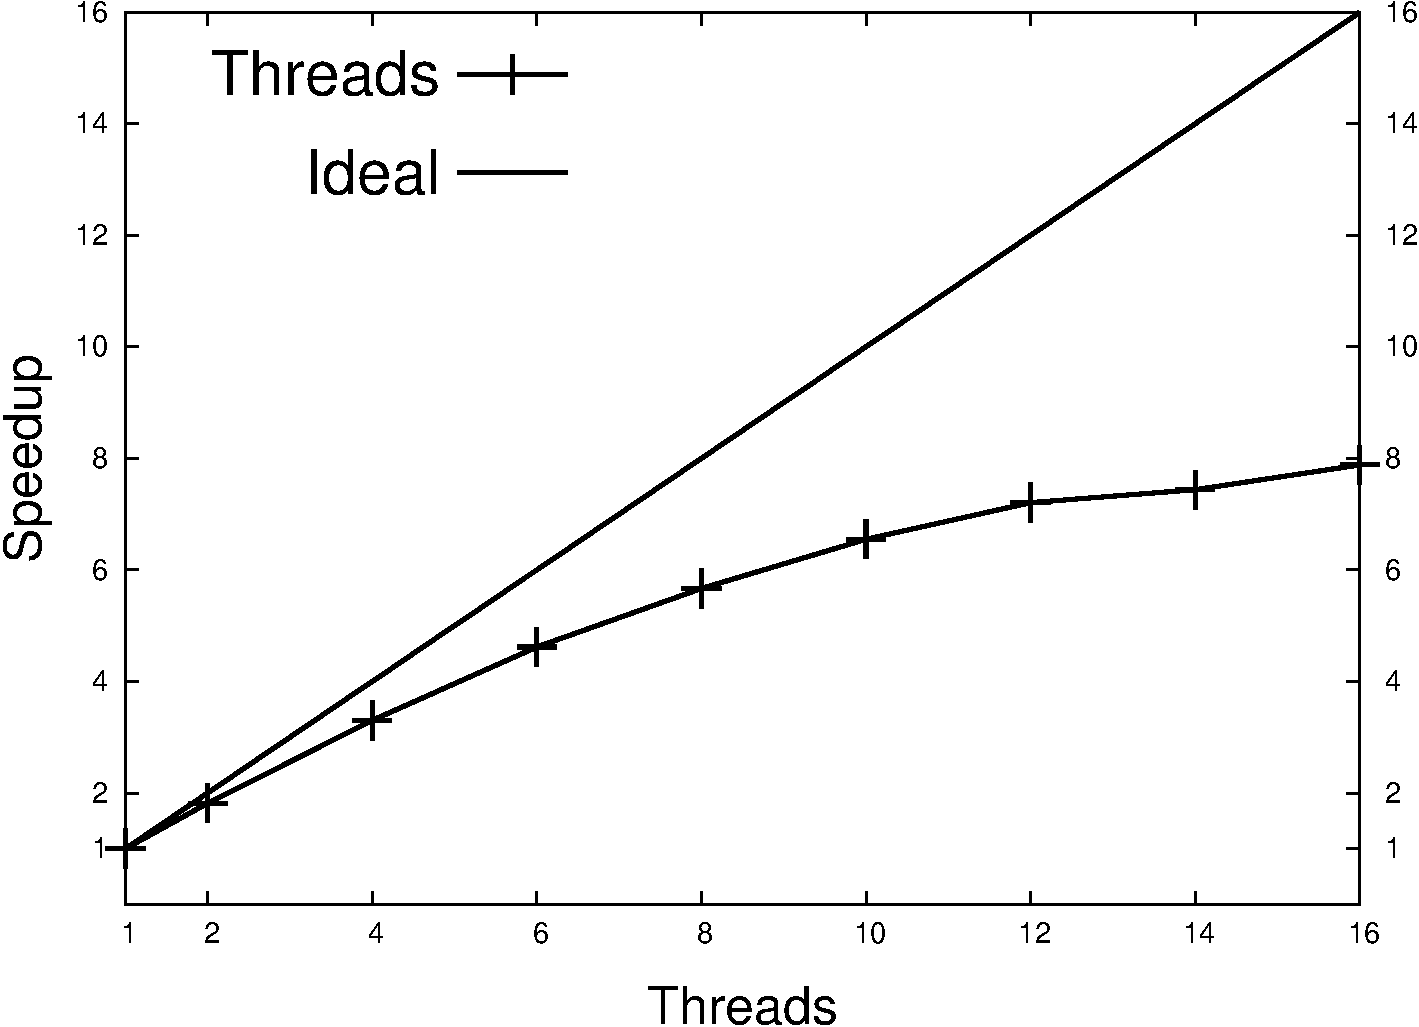
\includegraphics[width=\textwidth]{speedup_greedy-graph-coloring-2000.pdf}
      \caption{Using a random graph with 2,000 nodes and 600,000 edges.\newline}
   \end{subfigure}
   \caption{Experimental results for the GGC algorithm.}
   \label{exp:graph_coloring}
   \vspace{-0.1\intextsep}
\end{figure*}

The PageRank results are shown in Fig.~\ref{exp:pagerank}. We used the same search engine dataset as before and a new random dataset with 5,000 nodes and 500,000 edges. Although the search engine graph (Fig.~\ref{exp:pagerank}a) has half the edges (around 250,000), it scales better than the random graph (Fig.~\ref{exp:pagerank}b), meaning that the PageRank program depends on the number of nodes to be more scalable.

\begin{figure*}[h]
   \vspace{-0.1\intextsep}
   \centering
   \begin{subfigure}[b]{\plotsize}
      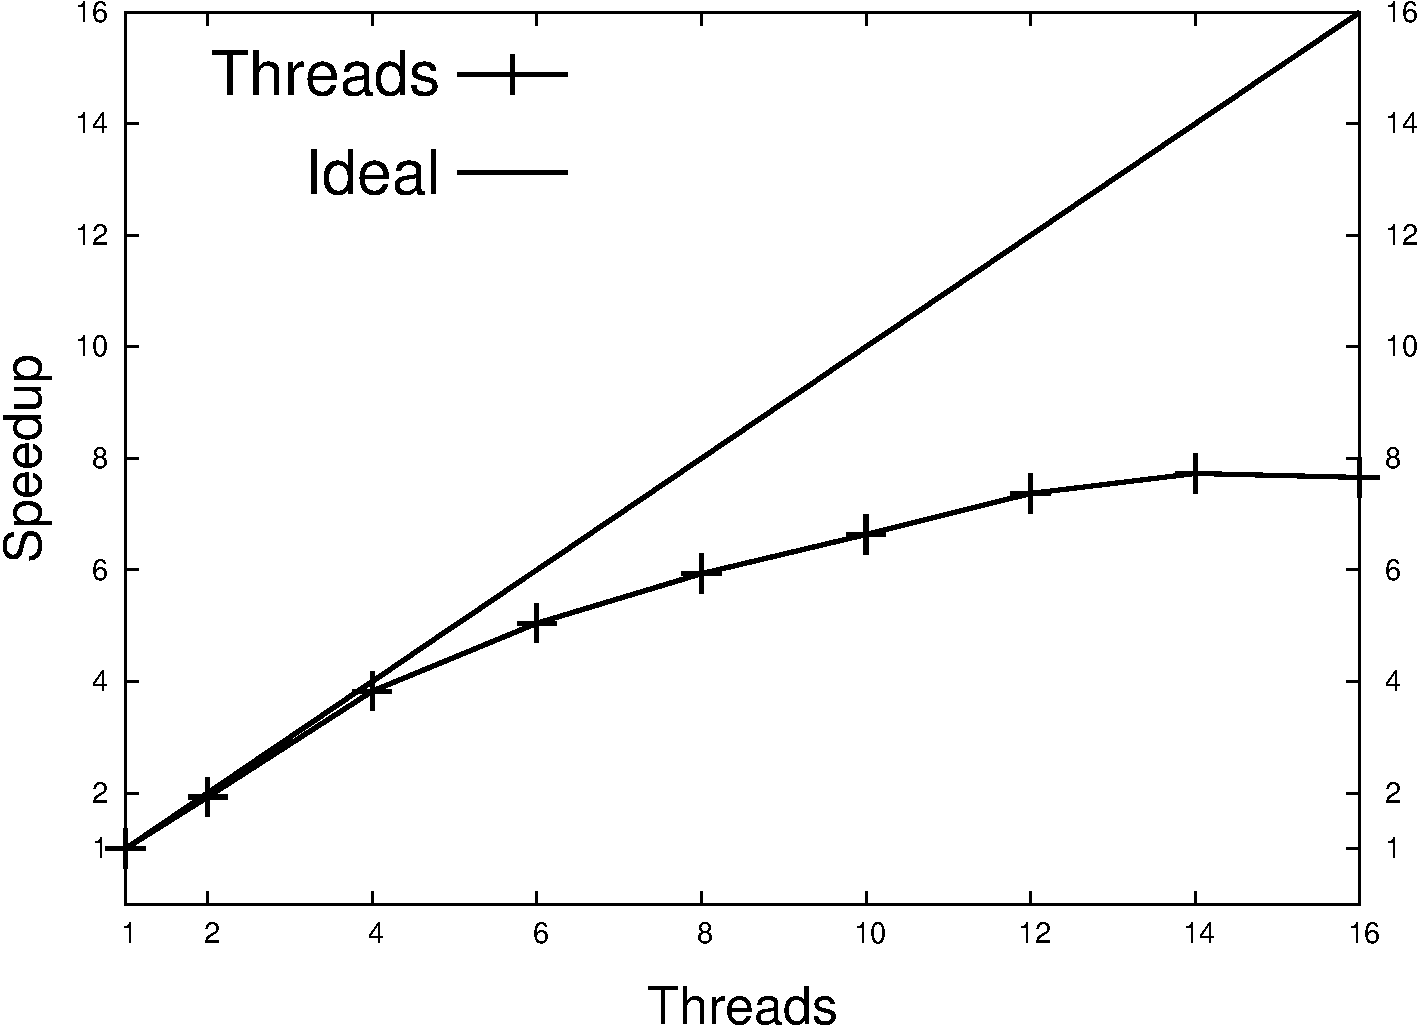
\includegraphics[width=\textwidth]{speedup_pagerank-search_engines.pdf}
      \caption{Using a graph of web pages collected from a search engine (around 12,000 nodes and 292,000 edges)}
   \end{subfigure}
   ~~~~
   \begin{subfigure}[b]{\plotsize}
      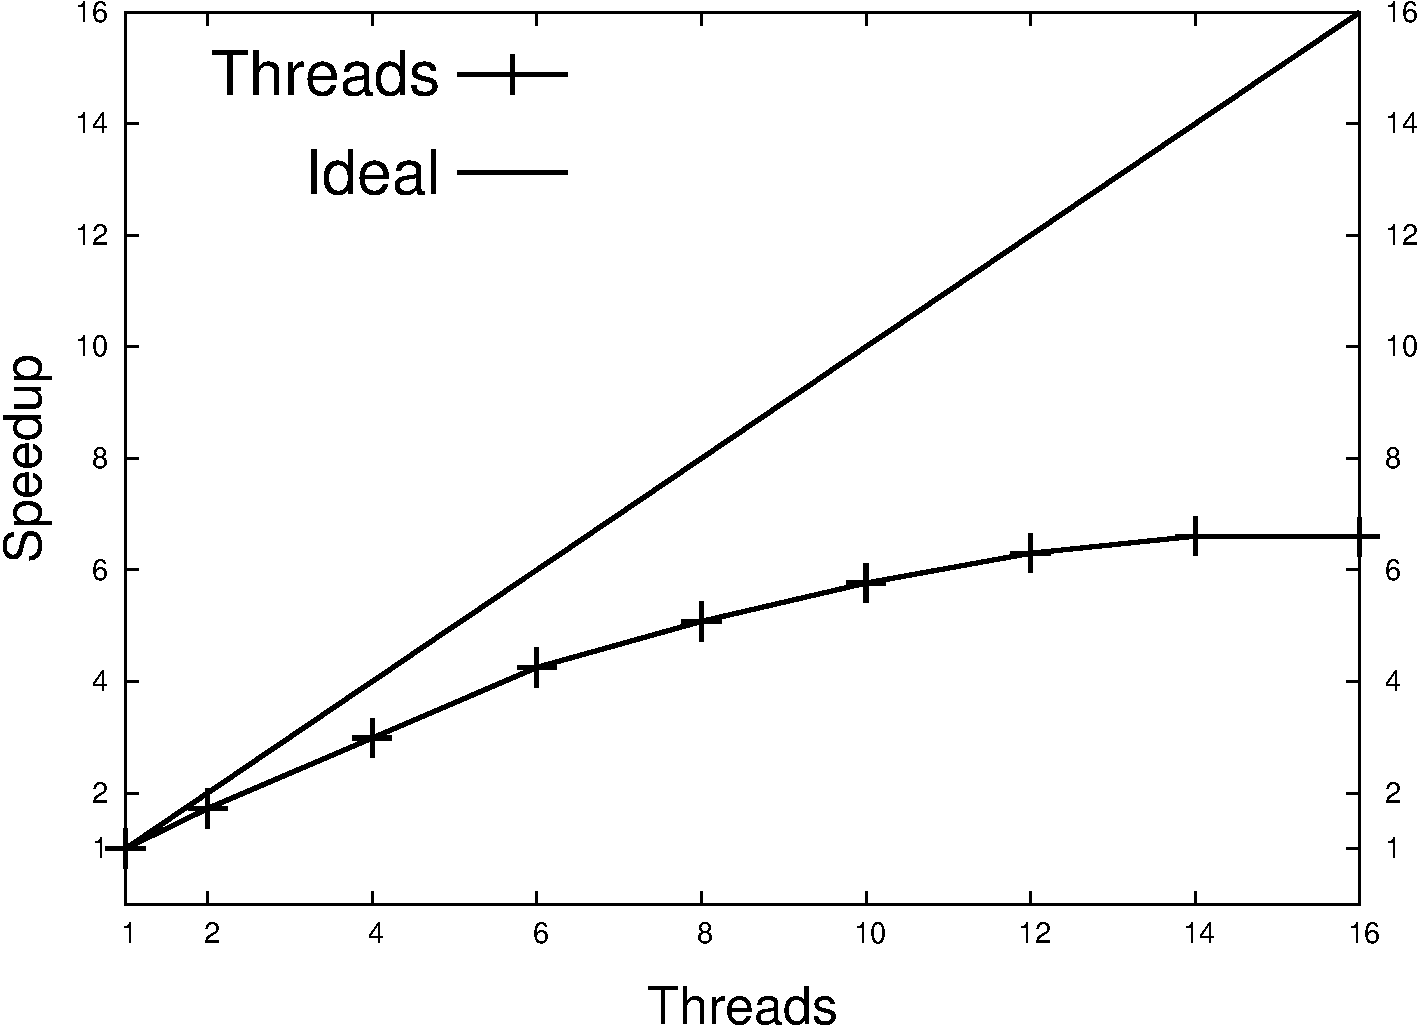
\includegraphics[width=\textwidth]{speedup_pagerank-5000.pdf}
      \caption{Using a random graph with 5,000 nodes and 500,000 edges.\newline}
   \end{subfigure}
   \caption{Experimental results for the asynchronous PageRank algorithm.}
   \label{exp:pagerank}
   \vspace{-0.8\intextsep}
\end{figure*}

The results for the N-Queens program are shown in Fig.~\ref{exp:8queens}. The program is not regular since computation starts at the top of the grid and then rolls down, until only the last row be doing computation. Because the number of valid states for the nodes in the upper rows is much less than the nodes in the lower rows, this may potentially lead to
load balancing problems. The results show that our system is able to scale well due to work stealing.

\begin{figure*}[h]
   \vspace{-0.7\intextsep}
   \centering
   \begin{subfigure}[b]{\plotsize}
      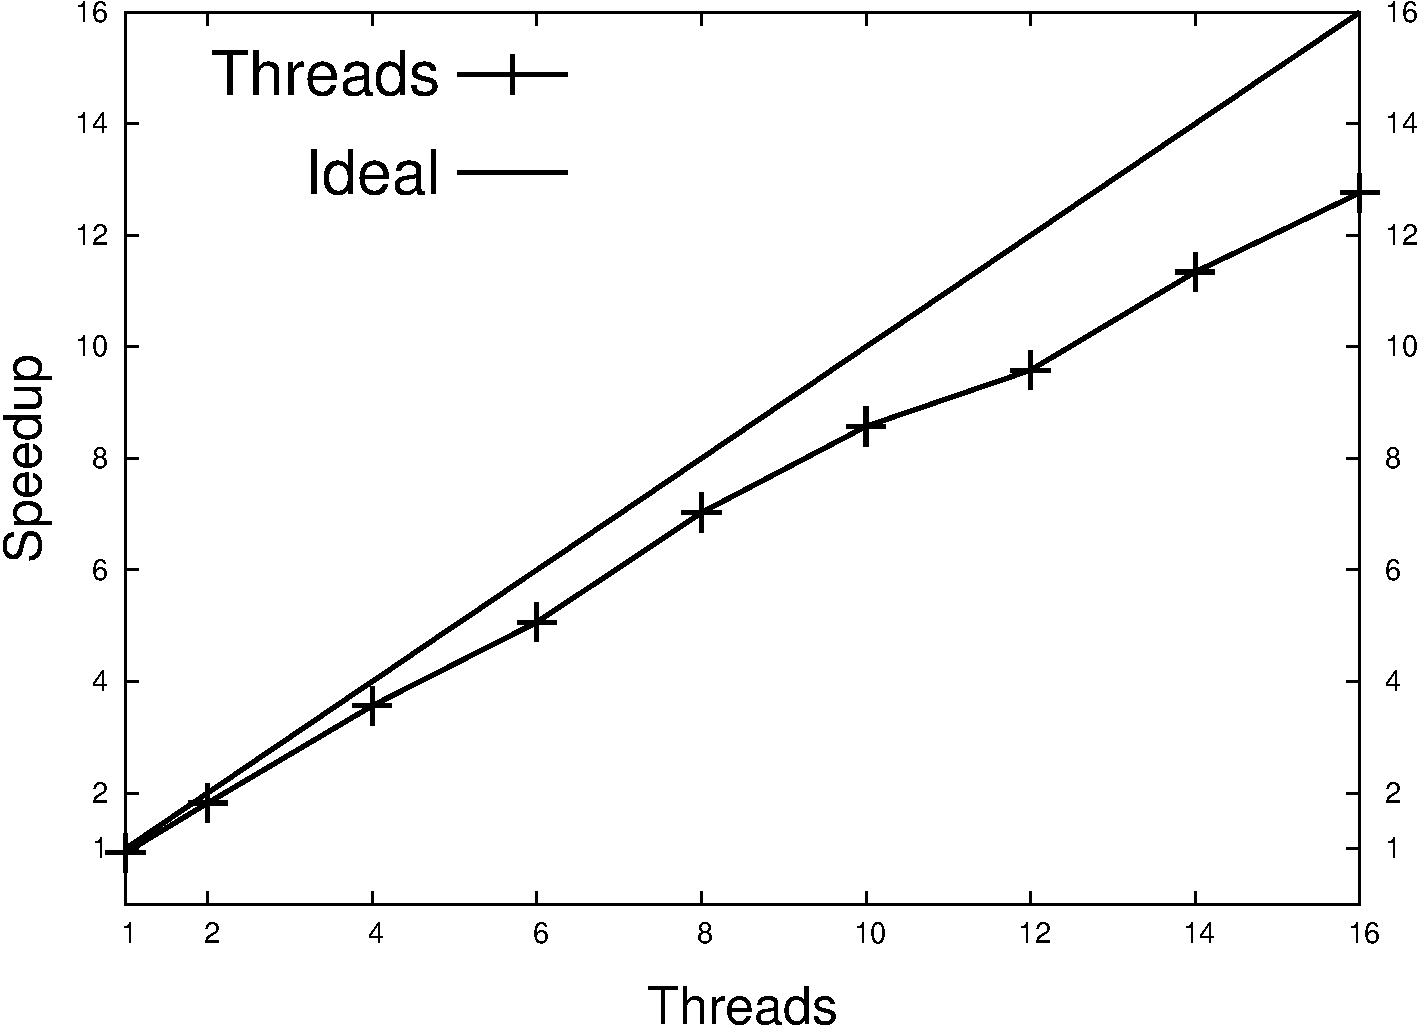
\includegraphics[width=\textwidth]{speedup_8queens-13.pdf}
      \caption{N-Queens program (13x13~board).}
      \label{exp:8queens}
   \end{subfigure}
   ~~~~
   \begin{subfigure}[b]{\plotsize}
      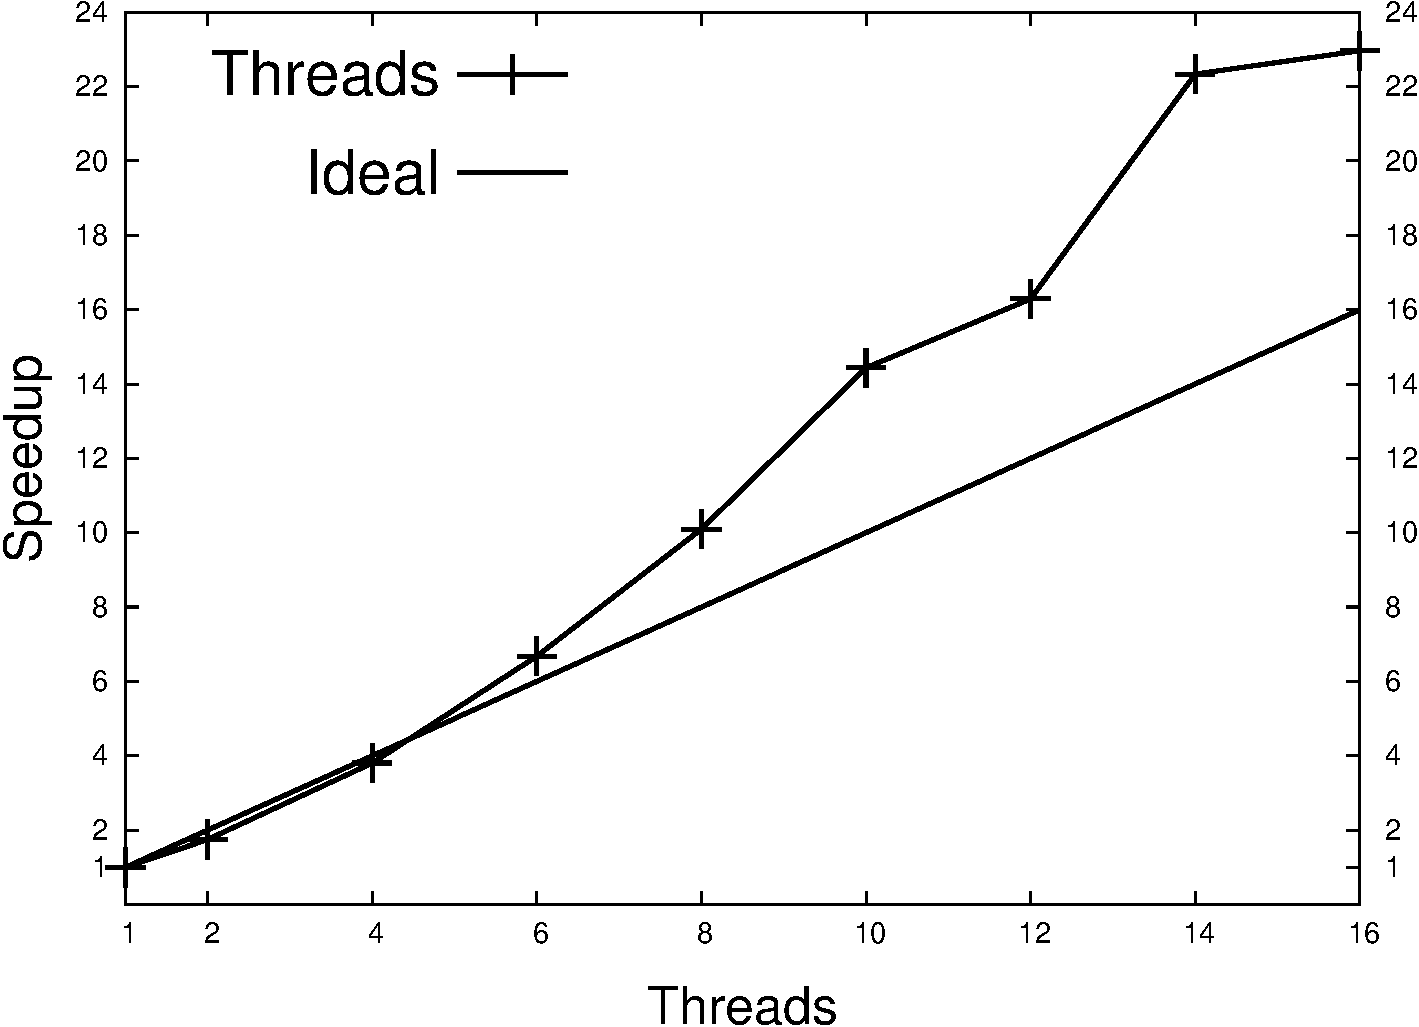
\includegraphics[width=\textwidth]{speedup_bp-400.pdf}
      \caption{BP (400x400~image).}
      \label{exp:bp}
   \end{subfigure}
   \caption{Experimental Results for N-Queens and Belief Propagation.}
   \vspace{-0.1\intextsep}
\end{figure*}

Finally, we shown the results for the Belief Propagation~(BP) program in Fig.~\ref{exp:bp}. BP is a regular and asynchronous program
and benefits (as expected) from having multiple threads executing since the belief values of each node will converge faster.
The super-linear results prove this assertion.

\subsubsection{Absolute Execution Time}

As we have seen, our VM scales reasonably well, but how does it compare in terms of absolute execution time
with other competing systems? We next present such comparison for the execution time using one thread.

In Fig.~\ref{comp:nqueens} we compare the LM's N-Queens version against 3 other versions: a straightforward sequential program implemented
in C using backtracking; a sequential Python~\cite{vanRossum:1995:PRM}
implementation; and a Prolog implementation executed in
YAP Prolog~\cite{DBLP:journals/corr/abs-1102-3896}, an efficient implementation of Prolog. Numbers less than 1 mean that LM
is faster and larger than 1 mean that LM is slower. We see that LM easily beats Python, but is 5 to 10 times slower than YAP
and around 15 times slower than C.
However, note that if we use at least 16 threads in LM, we can beat the sequential implementation written in C.

\begin{figure*}[h]
   \vspace{-0.1\intextsep}
   \centering
   
   \begin{subfigure}[b]{0.45\textwidth}
      \resizebox{5cm}{!} {
      \begin{tabular}{ | l | l | l | l |}
       \hline

       Size & C & Python & YAP Prolog \\ \hline\hline
       10 & 16.92 & \textbf{0,62} & 5,42 \\
       11 & 21.59 & \textbf{0.64} & 6.47 \\
       12 & 10.32 & \textbf{0.73} & 7.61 \\
       13 & 14.35 & \textbf{0.88} & 10.38 \\
       \hline
       \end{tabular}}
       \caption{N-Queens problem.}
      \label{comp:nqueens}
   \end{subfigure}
   ~~~~
   \begin{subfigure}[b]{0.45\textwidth}
      \resizebox{4.6cm}{!} {
      \begin{tabular}{ | l | l | l | l |}
       \hline

       Size & C & Python & GraphLab \\ \hline\hline
       10 & \textbf{0.67} & \textbf{0,03} & \textbf{1.00} \\
       50 & \textit{1.77} & \textbf{0.04} & \textit{1.73} \\
       200 & \textit{1.99} & \textbf{0.05} & \textit{1.79} \\
       400 & \textit{2.00} & \textbf{0.04} & \textit{1.80} \\
       \hline
       \end{tabular}}
       \caption{Belief Propagation program.}
       \label{comp:bp}
   \end{subfigure}
   \caption{Comparing absolute execution times (System Time / LM Time).}
   \vspace{-0.8\intextsep}
\end{figure*}

In Fig.~\ref{comp:bp} we compare LM's Belief Propagation program against a sequential C version, a Python version and a GraphLab version. GraphLab~\cite{GraphLab2010} is a parallel C++ library used to solve graph-based problems in machine learning. C and GraphLab
perform about the same since both use C/C++. Python runs very slowly since it is a dynamic programming language and BP has many
mathematical computations. We should note, however, that the LM version uses some external functions written in C++ in order
to improve execution time, therefore the comparison is not totally fair.

We also compared the PageRank program against a similar GraphLab version and LM is around 4 to 6 times slower.
Finally, our version of the all-pairs shortest distance algorithm is 50 times slower than a C sequential implementation of the Dijkstra algorithm, but it is almost twice as fast when compared to the same implementation in Python.

%\section{Related Work}\label{related_work}
%As a forward-chaining linear logic programming language, LM shares similarities with Constraint Handling Rules (CHR)~\cite{Betz:2005kx,Betz:2013:LBA:2422085.2422086,DBLP:journals/corr/abs-1006-3039}.
CHR is a concurrent committed-choice constraint language used to write constraint solvers. A CHR program is a set of rules and
a set of constraints (which can be seen as facts). Constraints can be consumed or generated during the application of rules.
Unlike LM, in CHR there is no
concept of rule priorities, but there is an extension to CHR that supports them~\cite{DeKoninck:2007:URP:1273920.1273924}.
Some optimizations ideas used in LM such as join optimizations and using different data structures for indexing facts
are inspired in research done in CHR~\cite{DBLP:journals/corr/cs-PL-0408025}.

There are also non logical based systems intended to solve graph-based problems such as Dryad, Pregel or GraphLab.
The Dryad system~\cite{Isard:2007:DDD:1272996.1273005} is a framework that combines computational vertices
with communication channels (edges) to form a data-flow graph. Each program is scheduled to
run on multiple computers or cores and data is partitioned during runtime. Routines that run on computational vertices
are sequential, with no locking required.
The Pregel system~\cite{Malewicz:2010:PSL:1807167.1807184} is also graph-based, although programs have a more strict
structure. They must be represented as a sequence of iterations where each iteration is composed of computation and message passing.
Pregel is aimed at solving very big graphs
and to scale to large architectures. GraphLab~\cite{GraphLab2010} is a C++ library for developing parallel machine learning algorithms. While
Pregel uses message passing, GraphLab allows nodes to have read/write access to different scopes through different concurrent access models in order to balance performance and data consistency. Each consistency model provides different guarantees that are suited to multiple classes of algorithms. GraphLab also provides several schedulers that dictate the order in which node's are computed.

\section{Conclusions}
We have presented the LM language and described how the VM is implemented, including
parallel scheduling on multicores, rule execution and database organization for fast insertion,
lookup, and deletion or linear facts.
Our preliminary results show that the VM is able to scale problems reasonably well when run with up to 16 threads.
Although this is still a work in progress, the VM fairs relatively well against other programming languages.
Moreover, since LM programs are executed in parallel, we can easily get better performance from the start by executing
the program with multiple threads.

In the future, we intend to take advantage of linear logic to perform whole-program optimizations,
including computing program invariants, loop detection in rules and bypass of rule priorities. For instance,
we want to detect during compile time which might be the best data structure for each predicate depending in how it
is used in the rules.

\bibliographystyle{splncs03}
\bibliography{refs}
\end{document}
